\documentclass[14pt]{extarticle}        
\usepackage[a4paper,				
        margins, a4
	    lmargin=2.5cm,rmargin=2cm,	
	    tmargin=2.5cm,			
	    bmargin=2cm,			
	    marginpar=1cm,			
	    marginparsep=0.5cm,			
	    headheight=17pt]{geometry}	
	    
\usepackage[utf8]{inputenc}			
\usepackage[english,russian]{babel}	
\usepackage[unicode=true,
	    colorlinks=true,
	    linkcolor=black]{hyperref}
	    
\usepackage{caption}
\usepackage{graphicx}				
\usepackage{tabu}				
\usepackage{xparse}				
\usepackage{titlesec}				
\usepackage{indentfirst}

\setlength{\parindent}{5ex}		
\setlength{\parskip}{0pt}
\clubpenalty=10000 \widowpenalty=10000	


\DeclareCaptionLabelFormat{rightparen}{#2)}
\captionsetup{labelsep=space,justification=justified,singlelinecheck=off}
\captionsetup[table]{labelsep=period,position=t,justification=raggedright,singlelinecheck=off,aboveskip=0pt}
\captionsetup[figure]{labelsep=period,justification=centering,singlelinecheck=off,aboveskip=10pt}

\renewcommand{\labelitemi}
	     {\normalfont\bfseries{--}}		
\renewcommand{\le}{\leqslant}
\renewcommand{\ge}{\geqslant}
\newcommand{\degC}{\(\,^{\circ}{\rm C}\)}

\newcolumntype{Y}[1]{>{\strut\hspace{0pt}}X[#1]<{\hspace{0pt}\strut}}
\tabucolumn Y
\renewcommand{\baselinestretch}{1.5}

\NewDocumentCommand{\rot}{O{90} O{1em} m}{\makebox[#2][l]{\rotatebox{#1}{#3}}}

\makeatletter

\newcommand{\titulnik}{
\begin{titlepage}
 \begin{center}
    Министерство образования и науки Российской Федерации\\
    Федеральное государственное бюджетное образовательное учреждение высшего образования\\
    Волгоградский Государственный Технический Университет\\
    Кафедра «Системы автоматизированного проектирования и поискового конструирования»
 \end{center}
 \vspace{2cm}
 \vbox{
  \hfill
  \parbox{7.5cm}{
   \centerline{УТВЕРЖДАЮ}
   \centerline{Зав. кафедрой САПР и ПК}\vspace{20pt}
   \hrulefill~д.т.н.\,~Щербаков М.В.\par\vspace{7pt}
   \centerline{
   \hbox to 6cm{<<\rule{7mm}{0.4pt}>>\hrulefill~\number\year\,г.}}
   }
  }
 \vfill
 \begin{center}
   Разработка модуля документооборота при получении канцтоваров и иных товаров от поставщиков\vspace{1cm}\\
    Техническое задание\\
    \MakeUppercase{15 листов}
 \end{center}
 \vfill
 \vfill
 \vfill
 \vspace*{1cm}
 \centerline{Волгоград, \number\year}
\end{titlepage}
\setcounter{page}{2}
}

\setcounter{secnumdepth}{5}
\renewcommand*{\thesection}{\arabic{section}}
\renewcommand*{\thesubsection}{\thesection.\arabic{subsection}}
\renewcommand*{\thesubsubsection}{\thesubsection.\arabic{subsubsection}}

\setlength{\parindent}{2em}
\titlespacing*{\subsection}{0pt}{15pt}{1em}
\titlespacing*{\subsubsection}{0pt}{15pt}{1em}
\titlespacing*{\paragraph}{0pt}{15pt}{1em}

\titleformat{\section}[block]{\normalfont}{\hspace*{\normalparindent}\thesection}{1em}{}
\titleformat{\subsection}[block]{\normalfont}{\hspace*{\normalparindent}\thesubsection}{1em}{}
\titleformat{\subsubsection}[block]{\normalfont}{\hspace*{\normalparindent}\thesubsubsection}{1em}{}
\titleformat{\paragraph}[block]{\normalfont}{\hspace*{\normalparindent}\theparagraph}{1em}{}

\begin{document}

\titulnik{}
	    
\newpage
\tableofcontents
\newpage

\section{Введение}
\label{sec:purpose}

\subsection{Наименование программы}
Наименование программы – «Разработка модуля документооборота при получении канцтоваров и иных товаров от поставщиков» под ОС Windows.

\subsection{Краткая характеристика области применения}
Областью применения программного продукта является любая сфера деятельности, связанная с закупками товаров. 

\newpage

\section{Основания для разработки}

\subsection{Основания для проведения разработки}
Основанием для проведения разработки является выдача задания на выпускную работу бакалавра и требование предоставить результаты до конца 07.03.2018. Задание выдано старшим преподавателем кафедры САПР и ПК Пеньковской Анной Петровной, именуемым в дальнейшем Заказчиком, и утвержден студентами Беззубцевым Иваном Алексеевичем, Немцевым Михаилом Алексеевичем именуемым в дальнейшем Исполнителями.

\subsection{Наименование темы разработки – «Разработка модуля документооборота при получении канцтоваров и иных товаров от поставщиков». Условное обозначение темы разработки (шифр темы) – «GS Module».} 

\newpage

\section{Назначение разработки}
\subsection{Функциональное назначение}
Функциональным назначением программы является автоматизация документооборота, связанного с закупкой канцтоваров и иных товаров по грантам.

\subsection{Эксплуатационное назначение}
Программа должна эксплуатироваться в профильных подразделениях на объектах заказчика, а также в свободном пользовании клиентов.

\newpage

\section{Требования к программе или программному изделию}
\subsection{Требования к функциональным характеристикам}
\subsubsection{Требования к составу выполняемых функций}
Программа должна обеспечивать возможность выполнения перечисленных ниже функций:\par
\begin{itemize} 
    \item функция внутреннего документооборота;
    \item функция электронной подписи;
    \item функция обмена документами между пользователями;
    \item шифрование документов.
\end{itemize}
\parДиаграмма бизнес процесса А.

\subsubsection{Требования к организации входных данных}
Входными данными являются отсканированные документы поставщика товаров, такие как счет и акт приемки.
  
\subsubsection{Требования к организации выходных данных}
Выходными данными является документы со всеми собранными подписями и печатями.

\subsection{Требования к надёжности}  
\subsubsection{Время восстановления после отказа}
Время восстановления после отказа, вызванного сбоем электропитания технических средств (иными внешними факторами), не фатальным сбоем (не крахом) операционной системы, неограниченно. 
\par Время восстановления после отказа, вызванного неисправностью технических средств, фатальным сбоем (крахом) операционной системы, неограниченно.

\subsubsection {Отказ из-за некорректных действий оператора}   
Отказы программы, в принципе, не возможны вследствие некорректных действий оператора (пользователя) при взаимодействии с операционной системой. 

\subsection {Условия эксплуатации}
\subsubsection {Климатические условия эксплуатации}
Климатические условия эксплуатации, при которых должны обеспечиваться заданные характеристики, должны удовлетворять требованиям, предъявляемым к техническим средствам в части условий их эксплуатации.

\subsection {Требования к численности и квалификации персонала}
Минимальное количество персонала, требуемого для работы программы, должно составлять не менее 2 штатных единиц – разработчика и пользователя программы.
\par Разработчик должен обладать навыками поддержания работоспособности программы, его обновления и дополнения.
\par В связи с простотой программы, пользователь должен без труда или же с последующим изучением, овладеть навыками использования данной программы.

\subsection {Требования к составу и параметрам технических средств}
\subsubsection {Требования к информационной и программной совместимости}
Хранение записей о грантах должно быть реализовано в виде реляционной базы данных.
\subsubsection {Требования к исходным кодам и языкам программирования}
Программа должна быть написана на языке программирования C#  посредством использования  Microsoft Visual Studio.

\subsubsection {Требования к программным средствам, используемым программой}
Программа будет оптимально работать на операционной системой Windows.

\subsection {Требования к маркировке и упаковке}
\subsubsection {Требования к маркировке}
Маркировка должна быть реализована в виде дополнительной страницы в приложении с возможностью открытия и просмотра пользователем. 
\par В данном разделе следует указать имя исполнителя (компании), номер версии программы и дату выпуска.

\subsection {Требования к транспортированию и хранению}
Готовая и протестированная программа передаётся на хранение и использование заказчику. 
\par Также оно хранится у исполнителя, который по возможности может дополнять и улучшать программу для более удобного функционирования.
\par Также программа может быть загружена на личный интернет-ресурс разработчика для дальнейшего скачивания и использования другими пользователями.

\subsection {Специальные требования}
Программа должна обеспечивать взаимодействие с пользователем посредством графического пользовательского интерфейса, разработанного согласно рекомендациям компании-производителя операционной системы.

\newpage

\section{Требования к программной документации}
\subsection {Предварительный состав программной документации}
Документация работы должна включать в себя следующее:
\begin{itemize} 
    \item ГОСТ 19.201-78 - техническое задание. Единая система программной документации.
\end{itemize}

\newpage

\section{Технико-экономические показатели}
Программа является бесплатной в распространении. При этом, имея некоторые аналоги в своём роде, она будет отличаться дополнительными функциями и может пригодиться при работе в различных областях.
\subsection {Экономические преимущества разработкии}
Разработка программы малозатратная и программа является бесплатной в распространении.

\newpage

\section{Стадии и этапы разработки}
\subsection {Стадии разработки}
Разработка должна быть проведена в 9 стадий:
\begin{itemize} 
    \item изучение предметной области;
    \item анализ методов решения задачи;
    \item разработка тз;
    \item разработка структуры бд;
    \item разработка графического интерфейса;
    \item разработка серверной части;
    \item разработка клиентской части;
    \item программная реализация;
    \item тестирование.
\end{itemize}

\newpage

\subsection {Содержание работ по этапам}
Таблица 1 – Содержание работа по этапам

\begin{tabular}{ | p{1cm} | p{7cm} | p{7cm} | }
\hline
Этап & Содержание работ & Результат  \\ \hline
1. & Изучить предметную область, составить примерный план разработки. & Первичное понимание предметной области, примерный план разработки. \\ \hline
2. & Проанализировать существующие методы решения подобных задач, определиться с языком программирования и используемыми фреймворками. & План разработки, список фреймоворков и языков программирования. \\ \hline
3. & Разработать ТЗ по ГОСТ 19.201-78. & Готовое ТЗ. \\ \hline
4. & Разработать структуру БД. & Готовая БД. \\ \hline
5. & Разработать графический интерфейс программы. & Готовый графический интерфейс. \\ \hline
6. & Разработать серверную часть программы. & Готовая серверная часть. \\ \hline
7. & Разработать клиентскую часть программы. & Готовая клиентская часть. \\ \hline
8. & Реализовать конечный продукт. & Готовая программа. \\ \hline
9. & Протестировать программу, исправить выявленные недочеты. & Протестированная программа, готовое к эксплуатации. \\ \hline
\end{tabular}

\section{Порядок контроля и приемки}
\subsection {Виды испытаний}
Предусмотренные испытания программы проводятся заказчиком, либо комиссией, формируемой заказчиком. При проверке правильности работы программы должны быть выполнены испытания проверки правильности всех действий. Под «правильностью» понимается отсутствие ошибок, недочётов, которые могут привести к критическому прекращению работы системы, либо просто к её некорректной работе.
\par Работа может быть возвращена исполнителю, после проведения испытаний в следующих случаях:
\begin{itemize} 
    \item Некорректно построено ТЗ;
    \item ТЗ полностью не соответствует разрабатываемой системе;
    \item Имеются ошибки в программе;
\end{itemize}
\par Исполнитель устраняет ошибки в недельный срок и предоставляет программу на повторную проверку.

\subsection {  Общие требования к приёмке работы}
\begin{itemize} 
    \item Предъявить заказчику готовое техническое задание заказчику необходимо заверить его, устранив или добавив пункты по своему желанию;
    \item согласование технического задания с заказчиком, устранение ошибок и подпись технического задания со стороны заказчика;
    \item готовая для сдачи работа, должна полностью соответствовать пунктам технического задания исключения возможны, но только при согласовании с заказчиком. 
\end{itemize}

\newpage

Приложение А \\
\par Диаграмма вариантов использования программы
\begin{figure}[h]
\begin{center}
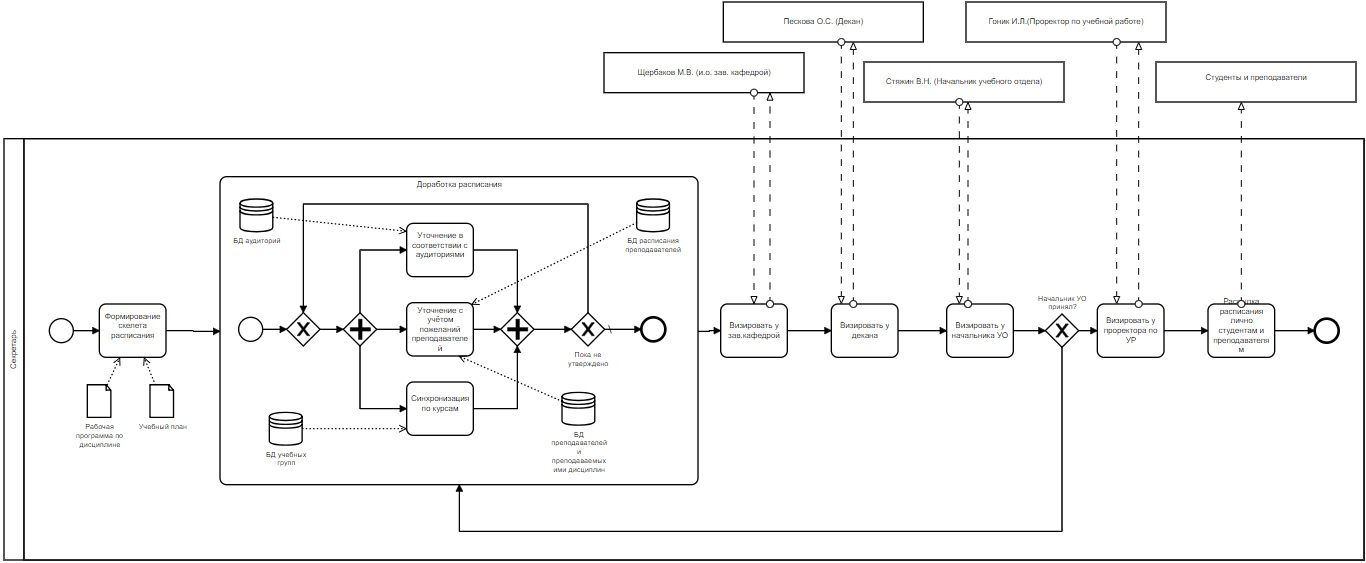
\includegraphics[width=500]{lab6}
\caption{Bpmn диаграмма бизнес процесса.}
\label{ris:experimoriginal} 
\end{center}
\end{figure}

\label{sec:purpose}
\end{document}
